Pour créer une interface mobile, il faut se mettre dans la peau de l'utilisateur, car une application mobile ne se conçoit pas comme un site web ou une application PC par exemple. Celle-ci va être utiliser en tactile avec un écran plus petit et de taille variable.


En suivant l'architecture de l'application, nous avons donc crée l'interface utilisateur. Celle-ci est disponible en annexe, ce n'est pas le design final mais la structure, elle oui.

\begin{figure}[H]
\begin{center}
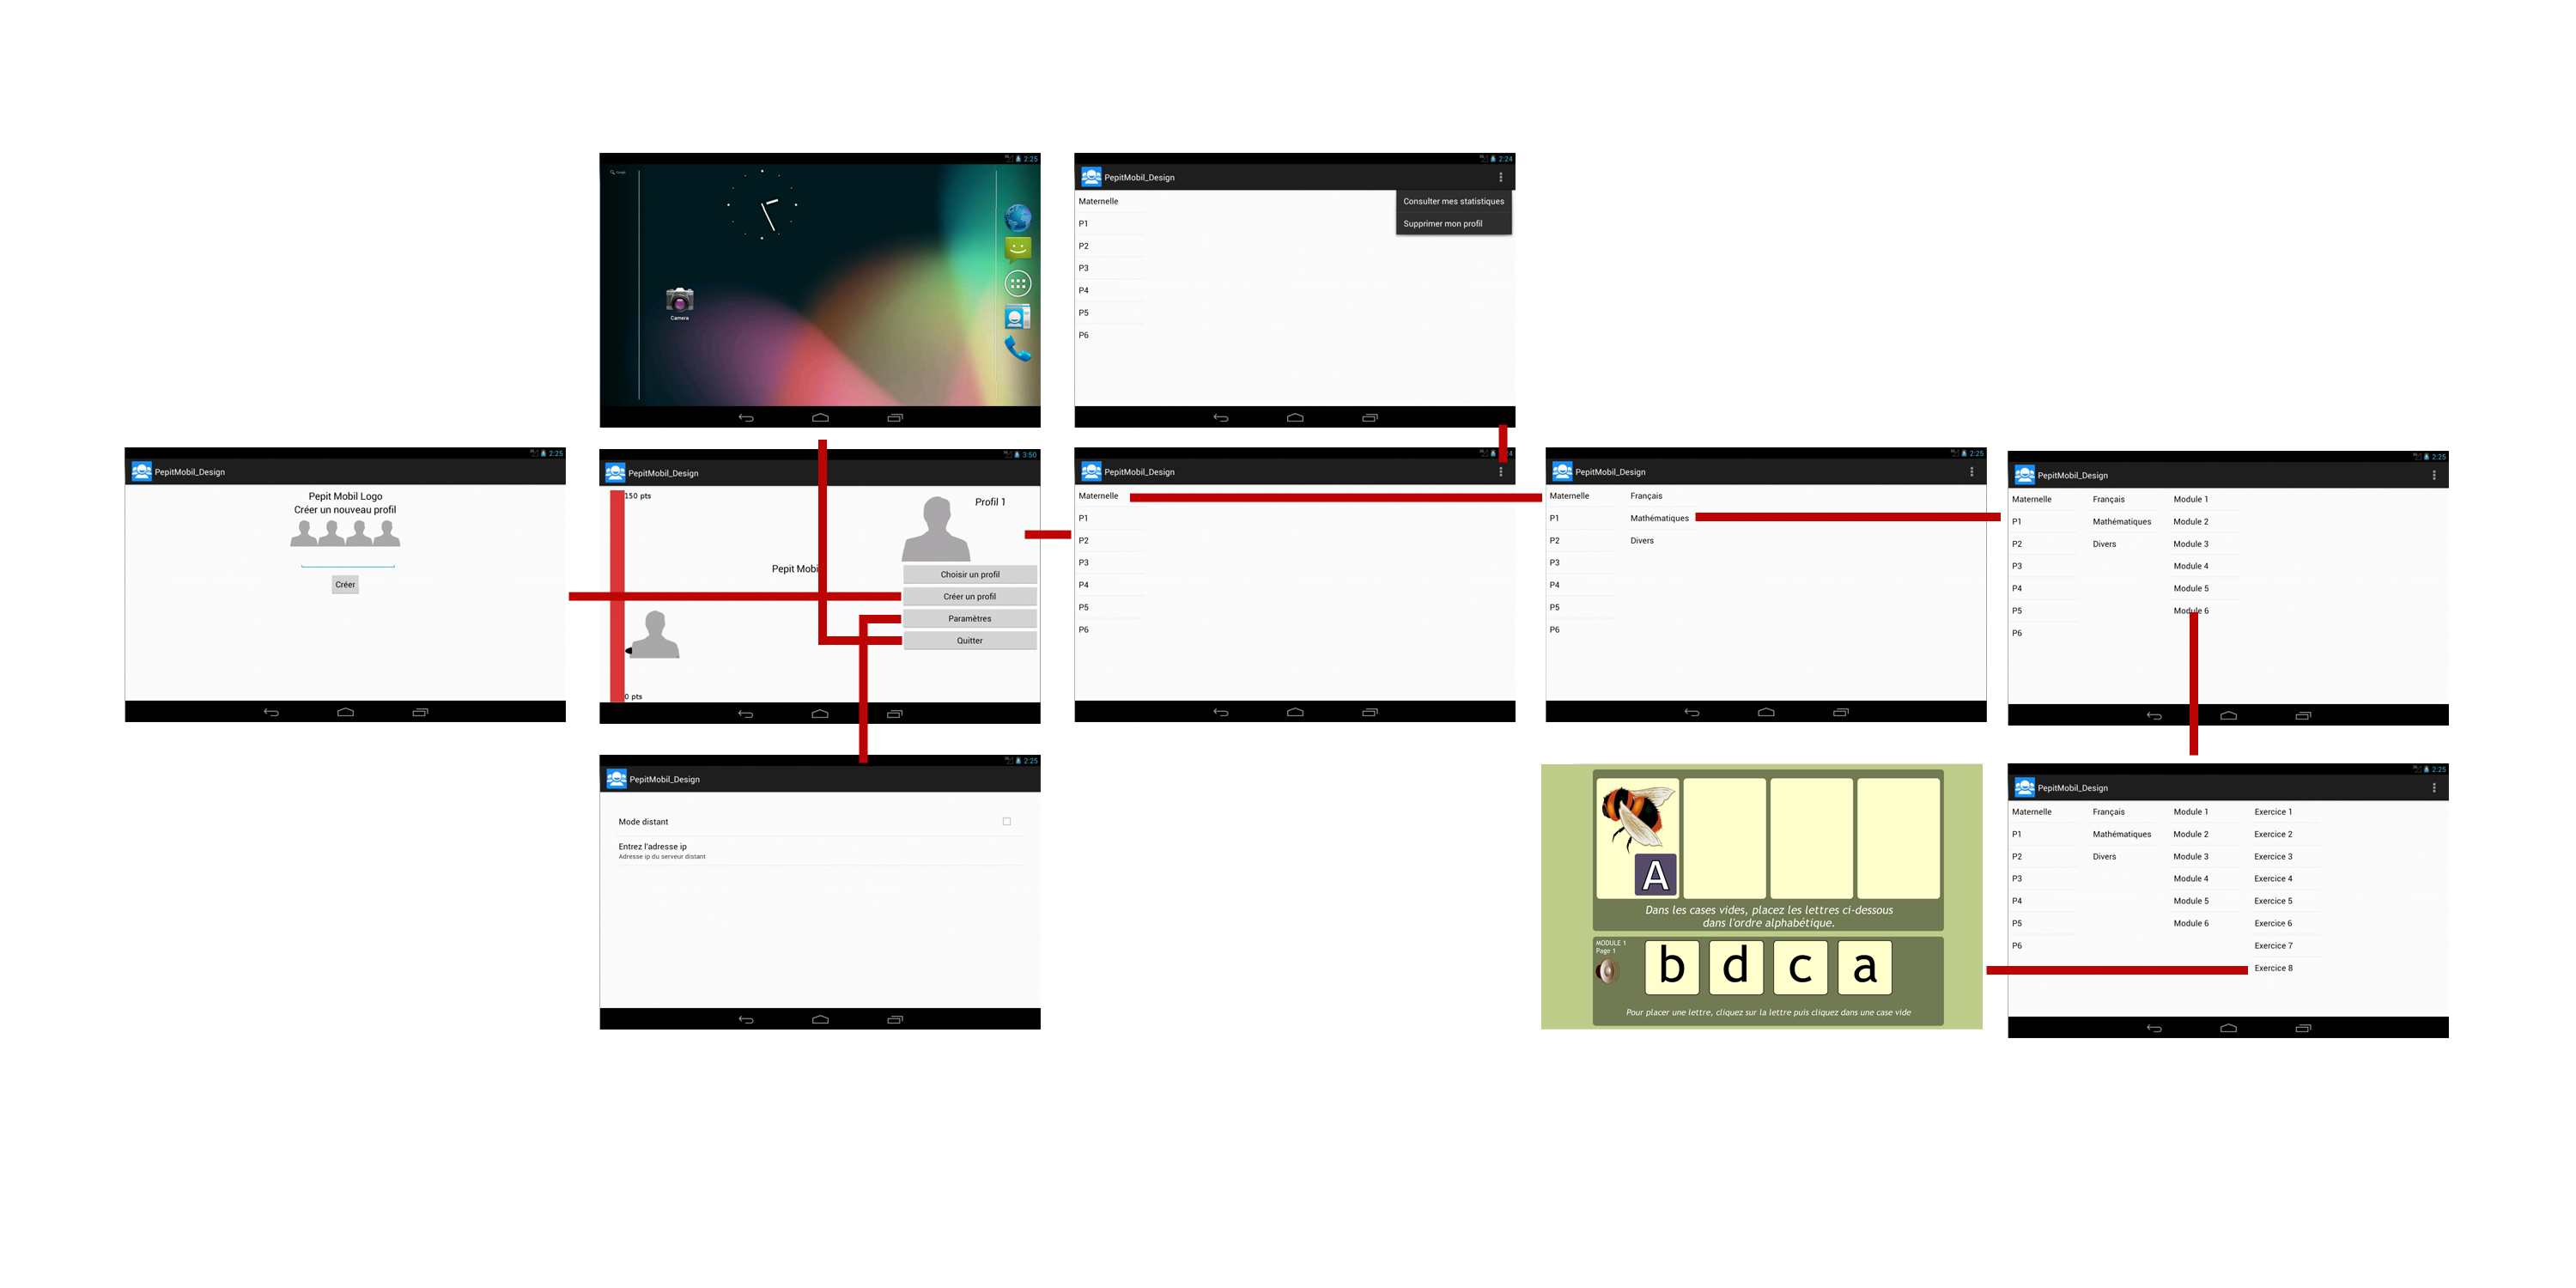
\includegraphics[width=15cm]{images/pepit_wireframe}
\end{center}
\caption{Maquettes de l'application}
\label{Maquettes de l'application}
\end{figure}